\section{Von der Datenbeschaffung zum fertigen Index}
\label{chap:data_aqcuisition}

Die in einer Dokumentensammlung enthaltenen Informationen bestimmen die Sinnhaftigkeit
einer Suchmaschine basierend auf diesen Dokumenten in besonderem Maße~\cite{croft.chap3}.
Dementsprechend stellt eine geeignete, mit vertretbarem Aufwand durchführbare,
Erzeugung dieser Dokumentensammlung den Anfang der Wertschöpfungskette dar.

Die im Kontext von Web-Suchmaschinen dafür benötigten Programme werden Crawler genannt~\cite{croft.chap3}.
Diese beschäftigen sich damit, Webseiten zu finden und herunterzuladen, um sie für spätere Verarbeitungsschritte lokal Verfügbar zu haben.
Die in der \hyperref[sec:intro]{Problembeschreibung} dargestellte Beschränkung auf die Website der Universität Leipzig
vereinfacht dieses, im Allgemeinen sehr anspruchsvolle, Problem und wird als Site Search bezeichnet~\cite{croft.chap2}.

Im Rahmen dieser Arbeit wurde zur Erzeugung der Dokumentensammlung die Freie Software~\cite{wiki.free_license}
Apache Nutch\footnote{Nutch ist~\href{https://github.com/apache/nutch/blob/master/LICENSE.txt}{unter Apache Version 2.0 lizensiert}.}
verwendet.
Nutch übernahm dabei sowohl die Aufgaben eines Crawlers\footnote{Der finale Crawling-Durchgang benötigte 14 Tage um 390 000 Dokumente in 50GB zu sammeln.}
als auch die unmittelbar folgenden Schritte bis einschließlich der Indexerzeugung.
Im folgenden werden verschiedene, während der Arbeit angewandten Anpassungen und Vereinfachungen des von Nutch bereitgestellten
Workflows vorgestellt.
 
\subsection{Domänenspezifische, manuell gepflegte Selectivity}
Unter den Features, die ein Crawler umsetzen sollte~\cite{manning.chap20},
findet sich auch die Notwendigkeit, die Qualität der zu crawlenden Seiten
in die Crawling-Reihenfolge einfließen zu lassen.
Am Beispiel von Nutch ist diese Funktionalität durch eine Bewertung der einzelnen Seiten
auf Basis der aktuell bekannten Linkstruktur realisiert~\cite{nutch.invert_links}.
Dabei werden Seiten, welchen eine höhere Wichtigkeit vorhergesagt wird, zeitiger heruntergeladen.

Aufgrund begrenzter Ressourcen wurde diese Idee weiter verschärft,
so dass bestimmte Seiten erst gar nicht gecrawlt wurden.
Dies betrifft Seiten, welche nicht direkt zur Universität gehören,
sowie Spider-Traps\footnote{Zum Beispiel ein
\href{http://www.informatik.uni-leipzig.de/~meyer/?d=15}{Kalender mit dynamisch erzeugten Links}.},
umfangreiche Webanwendungen\footnote{Zum Beispiel die 
\href{http://wortschatz.uni-leipzig.de/de}{Wortschatz}-, verschiedene 
\href{http://www.informatik.uni-leipzig.de/~duc/TD/td/index.php?bpos=72&db=ev}{Wörterbuch}-, oder auch
\href{http://pcai003.informatik.uni-leipzig.de/kosemnet/}{Semantic-Web}-Anwendungen.},
oder auch vollständige Suchmaschinen\footnote{Zum Beispiel ein
\href{http://lips.informatik.uni-leipzig.de/}{Dokumentenserver für Abschlussarbeiten}.} innerhalb der Universität.

Insbesondere für die letzteren besteht die Herausforderung darin,
genug Informationen über Existenz und Einsatzzweck einer solchen Seite zu sammeln,
ohne gleichzeitig unnötig vielen dynamisch erzeugten Links zu folgen.
Beispiel~\ref{example:document_server} beschreibt dies am Fall eines Dokumentenservers.

\begin{example}[Dokumentenserver FMI]{example:document_server}
	Der \href{http://lips.informatik.uni-leipzig.de/}{Dokumentenserver der Fakultät für Mathematik und Informatik}
	stellt unter anderem folgende Funktionalitäten bereit:

	\textbf{Den Download von Dokumenten:}\\
	Ein Nutzer kann die im Dokumentenserver enthaltenen Dokumente herunterladen.
	Dazu besitzt jedes Dokument eine Übersichtsseite, welche Metadaten zum Dokument bereitstellt sowie
	einen Link zum vollständigen Dokument.
	Beispiele dafür sind:
	\begin{itemize}
		\item Eine Übersichtsseite: \url{http://lips.informatik.uni-leipzig.de/pub/2017-0}
		\item Ein Dokument: \url{http://lips.informatik.uni-leipzig.de/files/thesis.pdf}
	\end{itemize}
	Beide enthalten wichtige Informationen und sollten gecrawlt werden.

	\textbf{Das Filtern nach Dokumenten:}\\
	Ein Nutzer kann über eine Facettensuche~\cite{wiki.facetted_search} innerhalb der Dokumente filtern.
	Beispiele dafür sind:
	\begin{itemize}
		\item Filterung nach \glqq Organisation IfI\grqq: \url{http://lips.informatik.uni-leipzig.de/browse/results/taxonomy%3A912}
		\item Filterung nach \glqq Organisation IfI und Author Erhard Rahm\grqq:\\ \url{http://lips.informatik.uni-leipzig.de/browse/results/taxonomy%3A912%20field_authors%3A%22Rahm%2C%20Erhard%22}
	\end{itemize}
	Die enorme Menge an möglichen Filter-Permutationen,
	sowie \href{http://se-pubs.dbs.uni-leipzig.de/pubs/results/0%200%200%200%20taxonomy%3A30%2C696}
		{teilweise auftretenden Endlosschleifen} lassen den Aufwand für ein Crawling dieser Seiten als unangemessen erscheinen.
	Dies wird abgerundet durch den Umstand, dass die oben beschriebenen Zielseiten ohne Filterung erreichbar sind.
	Dazu ist eine Traversierung von folgenden Seiten sinnvoll:
	\begin{itemize}
		\item Die erste Seite einer Liste aller vorhandenen Dokumente: \url{http://lips.informatik.uni-leipzig.de/browse/results/}
		\item Für welche nachfolgende Seiten direkt über Links zugänglich sind:
		\url{http://lips.informatik.uni-leipzig.de/browse/results?page=4}
	\end{itemize}
\end{example}

Um derartige Problemfälle zu behandeln müssen diese im ersten Schritt identifiziert werden.
Diesbezüglich bietet es sich an, während kleinerer Probe-Crawlings eine Auswertung der Logs vorzunehmen.
Um dies in vereinfachter Form durchzuführen,
wurde ein Statistik-Plugin für Nutch implementiert\footnote{Das Statistik-Plugin kann in dem
\href{https://github.com/DaniloMorgado/url_statistic_plugin}{entsprechenden Github-Repository} eingesehen werden.}.
Dieses Plugin identifiziert mittels
Map-Reduce\footnote{Einführungen in das Map-Reduce-Paradigma können hier eingesehen werden: \cite{wiki.mapreduce},
\cite{nosql.mapreduce}, \cite{hadoop.mapreduce}.}
Bereiche für die der Crawler besonders aktiv wird.
Dazu werden alle bekannten URLs durch Entfernung
von Queries oder Fragmenten normalisiert, und in ihre Bestandteile wie Schema, Host und Pfad zerlegt.
Beispiel~\ref{example:statistic_plugin} zeigt für die in
Beispiel~\ref{example:document_server} besprochenen Links,
wie durch aufsummieren dieser Bestandteile die Ausgabe des Plugins erzeugt wird.

\begin{example}[Berechnungsschritte des Statistik-Plugins]{example:statistic_plugin}
Die Map-Phase nimmt die Normalisierung der Links, sowie eine Umwandlung in die hierarchischen Bestandteile vor: \textbf{TODO MAIK BEISPIEL}

Die Reduce Phase summiert alle eintreffenden Paare bestehend aus Link-Bestandteil und count: \textbf{TODO MAIK BEISPIEL}
\end{example}
	
In der Ausgabe des Statistik-Plugins können schließlich sinnvoll Problemfälle identifiziert
werden\footnote{Neben den in Beispiel~\ref{example:document_server} hervorgehobenen Problemen sei hier noch auf potentiell fehlende Seiten hingewießen.
Diese können durch einen Vergleich der aufsummierten Linkbestandteile mit der Anzahl der von Google indexierten Seiten entdeckt werden.}.
Um dies effizient durchführen zu können,
bietet es sich an, dieses Plugin als Eingabe für existierende Standardwerkzeuge zu nutzen.
So erlaubt die nach Anzahl sortierte sowie durch einen Mindest-Threshold und White-List gefilterte Ausgabe
auf den ersten Blick potentielle Probleme zu identifizieren.

Im nächsten Schritt ist es notwendig, diese Problemfälle zu behandeln.
Eine einfache, aber effiziente, Möglichkeit, dies umzusetzen, wird in Nutch in Form von \href{https://github.com/apache/nutch/blob/master/conf/regex-urlfilter.txt.template}{Regex-Url-Filtern} bereitgestellt.
Darunter versteht man eine Liste von requlären Ausdrücken, welche jeweils um eine positive oder negative Markierung erweitert sind.
Für eine URL werden die regulären Ausdrücke dann der Reihe nach ausgewertet.
Der erste passende Ausdruck entscheidet, ob eine URL gecrawlt werden darf (falls der zugehörige Ausdruck positiv markiert ist),
oder nicht\footnote{Aus diesem Grund ist es üblich, 
die Liste der Ausdrücke mit einem entsprechendem immer zutreffendem Eintrag abzuschließen.}.

Die in Nutch vordefinierten Regex-Url-Filter verfolgen das Ziel,
das Crawling auf sinnvolle Protokolle\footnote{HTTP, kein mailto- oder file-Protokoll.}
und Dokument-Typen\footnote{Html-Seiten, keine CSS-Resourcen, Bilder oder Videos.} zu beschränken.
Um diese Filter systematisch korrekt zu erweitern wurde ein
Testgetriebenes Vorgehen gewählt\footnote{Die Implementierung findet
sich in dem Github-Repository \href{https://github.com/mam10eks/check-nutch-regex-urlfilter}{check-nutch-regex-urlfilter}.}.
Dieses zeichnet sich durch die Möglichkeit aus, einzelne Bereiche getrennt voneinander zu konfigurieren, ohne ungewünschte Seiteneffekte zu erwarten.

Nach dem \href{https://de.wikipedia.org/wiki/Teile-und-herrsche-Verfahren}{Teile-und-herrsche-Verfahren} werden
diesbezüglich für kleine Bereiche der zu crawlenden Webseiten einzeln anhand von Beispielen Konfigurationen vorgenommen.
Dafür werden für diesen Bereich Positiv- und Negativ-Beispiele in Form von Urls zusammengetragen.
Im nächsten Schritt werden die für diese Beispiele passenden Regex-Url-Regeln aufgestellt.
Diese verfolgen das Ziel, dass sie sich für alle Positivbeispiele zu positiv auswerten, und für alle Negativbeispiele entsprechend zu negativ.
Beispiel~\ref{example:regex_url} verdeutlicht dies für die aus Beispiel~\ref{example:document_server} bekannten Urls.

\begin{example}[Erstellung der Regex-Url-Regeln für den Dokumentenserver]{example:regex_url}
\# Positivbeispiele: Stelle sicher, dass die Dokumente gecrawlt werden\\
http://lips.informatik.uni-leipzig.de/browse/results?page=4\\
http://lips.informatik.uni-leipzig.de/files/thesis.pdf\\
http://lips.informatik.uni-leipzig.de/pub/2017-0

\# Negativbeispiele: Verhindere, dass die Filterfunktion genutzt wird\\
http://lips.informatik.uni-leipzig.de/browse/results/taxonomy%3A912

\# Regex-Url-Regeln, welche diese Anforderungen erfüllen\\
+http://lips.informatik.uni-leipzig.de/(pub|files)/.*\\
+http://lips.informatik.uni-leipzig.de/browse/results.*\\
-http://lips.informatik.uni-leipzig.de.*\\
\end{example}

Die Konfigurationen der einzelnen Bereiche werden schließlich \href{https://de.wikipedia.org/wiki/Top-down_und_Bottom-up}{Bottom-up} zu einer einzigen 
Url-Filter-Liste vereinigt.
Für diese Liste werden anschließend alle Positiv- und Negativ-Beispiele evaluiert.
Nur wenn dabei für alle Beispiele das spezifizierte Verhalten beobachtet wird, ist diese Url-Liste valide und kann verwendet werden.

Durch diese Hilfswerkzeuge wurde im Rahmen der Arbeit die Site der Universität Leipzig anhand ihrer Fakultäten auf die einzelnen Bearbeiter aufgeteilt.
Mit einer Reihe von Probe-Crawlings konnte die vollständige Regex-Url-Filter-Liste erstellt werden.
Mithilfe dieser Vorbereitung konnten die für den Index verwendeten Dokumente unterbrechungsfrei gecrawlt werden.
Dafür konnten die entstandenen Positiv-Beispiele direkt als \href{https://wiki.apache.org/nutch/NutchTutorial#Create_a_URL_seed_list-1}{Seeds} eingesetzt werden.

\subsection{Reproduzierbare Erzeugung eines Lucene Index mit Docker und Solr}

Um die gecrawlten Dokumente in der in Abschnitt~\ref{chap:ranking} beschriebenen Suchmaschine verfügbar zu machen, müssen sie in einen Lucene Index überführt werden.

Dafür wird im ersten Schritt eine sogenannte Conversion durchgeführt~\cite{croft.chap2}.
Dabei werden im vorliegenden Fall gecrawlte Dokumente,
welche in den unterschiedlichsten Formaten vorliegen können\footnote{Häufigstes Format war HTML, aber auch PDF, Word oder Power Point waren vertreten.}
in ein einheitliches Format umgewandelt.
Auf eine mögliche Reduzierung der Dokumente auf deren Main-Content wurde
verzichtet\footnote{Die Extraktion des Main-Content ist mit Apache Tika
unmittelbar möglich. Jedoch erschien es plausibel, dass für die gecrawlten Webseiten mit vergleichsweiße wenig Rauschen zu rechnen ist.}.
Realisiert wurde die Conversion mit \href{https://en.wikipedia.org/wiki/Apache_Tika}{Apache Tika}.

Anschließend wird mit Nutch eine \href{https://wiki.apache.org/nutch/bin/nutch_invertlinks}{Inversion der Links} durchgeführt.
Dabei werden für alle Dokumente die Texte der eingehenden Links in dedizierten Feldern an dem Dokument abgespeichert.
Im nächsten Schritt wird eine \href{https://github.com/apache/nutch/blob/master/src/java/org/apache/nutch/crawl/TextProfileSignature.java}{Near Duplicate Detection}
durchgeführt, welche näher in Abschnitt~\ref{chap:near_duplicate_detection} erläutert wird.

Nutch kann den Lucene Index nicht selbstständig erzeugen.
Aus diesem Grund wird mit einem \href{http://lucene.apache.org/solr/}{Solr Server} ein Index über die gecrawlten Dokumente erzeugt.
Diesbezüglich wird mit Solr eine Text Transformation~\cite{croft.chap2} durchgeführt.
Dabei wurde entsprechend der Standards auf eine Entfernung von Stoppwörtern sowie Stemming
verzichtet\footnote{Jedoch gehört das testen unterschiedlicher 
\href{https://github.com/apache/lucene-solr/blob/master/lucene/analysis/common/src/java/org/apache/lucene/analysis/core/StopFilterFactory.java}{Stoppwortlisten} sowie verschiedener
\href{https://github.com/apache/lucene-solr/blob/master/lucene/analysis/common/src/java/org/apache/lucene/analysis/en/PorterStemFilterFactory.java}{Stemmer}
zu dem geplanten Vorgehen,
die Effektivität der Suchmaschine für das durchgeführte Laborexperiment zu optimieren (Siehe Kapitel~\ref{chap:log_analysis}).}.
Die eigentliche Indexerzeugung mit Solr schließt diesen Prozess ab.
Dabei werden neben den Dokument-Statistiken~\cite{croft.chap2} für das spätere Scoring von Dokumenten auch Vorbereitungen zur Erzeugung von Snippets vorgenommen.
Der so erzeugte Index kann unmittelbar in Lucene eingesetzt werden.

Die hier beschriebene Erzeugung des Index aus den gecrawlten Dokumenten ist von vielen Parametern abhängig.
Dadurch wird eine häufige Wiederholung dieses Prozesses sinnvoll, um die Auswirkung von Anpassungen an verschiedenen Parametern zu prüfen.
Um den Aufwand dafür gering zu halten, wurde der komplette Workflow reproduzierbar automatisiert\footnote{Das
entsprechende Github-Repository mit
den Scripten und der Konfiguration ist \href{https://github.com/mam10eks/nutch_tools/}{Nutch-Tools}.}.

Dafür wird als Eingabe eine Menge von Nutch-Crawl-Directories erwartet.
Diese werden im ersten Schritt bereinigt, um ein erneutes Parsing der rohen Dokumente durchzuführen.
Danach werden die einzelnen, oben beschriebenen Arbeitsschritte durchgeführt.
Sobald die Indexerzeugung beginnt, wird der dafür notwendige Solr-Server mit Docker
bereitgestellt. Da die notwendige Konfiguration sowie das Index-Schema in den Container gemountet werden,
ist auch dieser Schritt einfach wiederholbar.

\subsection{Data Cleaning: Aggregation von Fast-Duplikaten}
\label{chap:near_duplicate_detection}

Duplikate und Fast-Duplikate treten in vielen Situationen auf~\cite{croft.chap3}.
Im Rahmen dieser Arbeit war die entsprechende Zielsetzung, diese transparent an den Nutzer zu kommunizieren.
Abbildung~\ref{fig:grouped_sim} stellt dies an einem Beispiel dar.

\begin{figure}[!ht]
	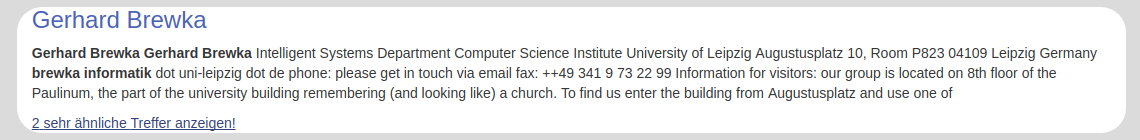
\includegraphics[width=0.99\textwidth]{chapter_data_aqcuisition/grouped_duplicates.png}
	\caption{Ein Dokument mit 2 Fast-Duplikaten}
	\label{fig:grouped_sim}
\end{figure}

\begin{wrapfigure}{H}{0.49\linewidth}
	\vspace*{-0.4cm}

\begin{scriptsize}
\begin{algorithm}[H]
	\SetKwInOut{Input}{Input}
	\SetKwInOut{Output}{Output}
		       
	\Input{ Document $\mathcal{D}$ }
	\Output{ Fingerprint for Document $\mathcal{D}$}

	TBA\\
	TBA\\
	TBA\\
	\caption{Text Profile}
	\label{alg:text_profile}
\end{algorithm}
\end{scriptsize}

	\vspace*{-0.2cm}
\end{wrapfigure}

Um dies zu ermöglichen, müssen zuerst die (Fast-)Duplikate identifiziert werden.
Dafür wurde das
\href{https://github.com/apache/nutch/blob/master/src/java/org/apache/nutch/crawl/TextProfileSignature.java}{TextProfileSignature}
-Verfahren verwendet.
Dieser Algorithmus weißt einem Dokument einen Fingerprint zu.
Dabei werden ähnliche Dokumenten auf den gleichen Wert abgebildet.
Algorithmus~\ref{alg:text_profile} zeigt dies im Pseudocode.
In Beispiel~\ref{example:text_profile} wird der Fingerprint für einen Text berechnet.

\begin{example}[Berechnung des Fingerprints mittels TextProfileSignature]{example:text_profile}

	\textbf{TODO MAIK}

\end{example}

Nach der Zuweißung des Fingerprints werden entsprechend dem Discovery Scenario alle Paare von Fast-Duplikaten
gesucht~\cite{croft.chap3}. Durch dieses Vorgehen entstehen Gruppen ähnlicher Dokumente.
Für jede solche Gruppe wird ein Repräsentant gewählt\footnote{Das längste Dokument wird der Vertreter.}.
Dieser wird um die Urls der anderen Gruppenmitglieder angereichert.
Abschließend werden die restlichen Dokumente einer Gruppe gelöscht\footnote{Die Implementierung ist in dem Modul 
\href{https://github.com/mam10eks/search-homepage-of-university-leipzig/tree/master/custom-index-cleaning}
{Custom Index Cleaning} zu finden.}.
